\section{电网络的基本定律}
\label{sec:electrical-network-laws}

把带正权边的无向图看成\term{电网络}（electrical network）：每条正权边是一个电阻元件，顶点是这些元件连接的接点，外部可以在指定接点注入或取出电流。我们先从一个接点看各条边的净流量，建立电流守恒方程；再从一条边看两端电势怎样决定流过它的电流，写出Ohm定律。

\subsection{电流守恒}
\label{sec:electrical-current-conservation}

一条边导电的容易程度用\term{电导}（conductance）$c_e = w_e > 0$来衡量，倒数$r_e = 1/c_e$是\term{电阻}（resistance）。电导越大，同样的电势差下流过的电流越多。零权边不导电，删去它们后保留的图称为正权支撑。正权支撑仍包括所有顶点，即使某个顶点不再与任何正权边相邻。

设顶点数为$n$，正权边数为$m$。每条边记录一个带符号的电流，组成向量$\bm f\in\mathbb R^m$。记录方向沿用第~\ref{chap:graph-incidence-matrix}章的约定：关联矩阵$\bm B\in\mathbb R^{n\times m}$的每列在尾端取$+1$、头端取$-1$。$f_e > 0$表示电流沿记录方向流动，$f_e < 0$表示实际流向与记录相反。

以四点图为例。边$41$的记录方向为$4\to1$。若边上流量为$-2$，实际含义是$2$个单位的电流从$1$流向$4$。看顶点$1$，这条边从外面带来了$2$个单位的电流。

每个顶点的进出必须平衡。由关联矩阵按行读取，顶点$i$在出发边上取$+f_e$，在到达边上取$-f_e$，各项相加得到净流出量$(\bm B\bm f)_i$。假设两条边的记录方向都朝外，其流量分别为$3$和$-1$。实际上前者送出$3$，后者从外面送入$1$，净流出$3 - 1 = 2$。

外部在顶点$i$注入电流$b_i$，这些电流必须从该点流向网络内部。$b_i > 0$是注入，$b_i < 0$是引出。\term{Kirchhoff电流定律}（Kirchhoff's current law）要求每个顶点的网络净流出等于外部注入：
\begin{equation}
  \bm B\bm f = \bm b.
  \label{eq:electrical-current-conservation}
\end{equation}
上面那个接点的净流出为$2$，所以外部恰好需要送入$b_i = 2$单位电流来维持平衡。

图~\ref{fig:electrical-local-current-balance}把同一个接点的电流守恒用两种方式画出来。左图用记录方向和带符号的数值。右图把方向转成实际流向，在接点处画出外部注入的量。

\begin{BookInlineFigure}
  \centering
  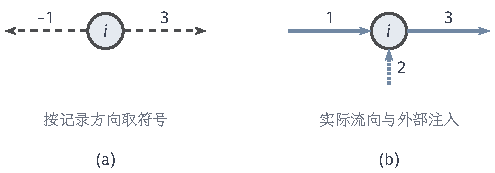
\includegraphics[scale=1]{figures/03-graphs/05-matrices-and-spectra/tikz/electrical-local-current-balance/figure.pdf}
  \caption{接点的电流守恒。(a)~虚线箭头给出两条边的记录方向，左边的负号表示逆向流动。(b)~两条实线箭头给出真实流向，下方点线箭头给出维持守恒所需的外部注入量。}
  \label{fig:electrical-local-current-balance}
\end{BookInlineFigure}

把式~\eqref{eq:electrical-current-conservation}的$n$个方程按顶点求和。每条边在尾端贡献$+f_e$，在头端贡献$-f_e$，两者抵消。因此全图的外部注入总和必须为零：
\[
  \sum_{i=1}^n b_i = \bm 1^\top \bm b = 0.
\]
对单个连通分量也一样——如果两个分量之间没有正电导边，电流就无法从一个分量穿越到另一个。每个正权连通分量必须各自满足注入总量为零。

\subsection{Ohm定律}
\label{sec:electrical-ohm-law}

守恒只限制流入和流出的总量，还没有决定每条边上有多少电流。每条边的电流由两端的电势差和该边的电导共同决定。

给每个顶点一个电势值$v_i$，组成向量$\bm v\in\mathbb R^n$。沿边$e\colon i\to j$看，电势从$v_i$变到$v_j$，沿记录方向的压降为$v_i - v_j$。例如$v_i = 3$、$v_j = 1$，压降为$2$。若这条边的电导为$c_e = 1/2$，\term{Ohm定律}（Ohm's law）给出流过它的电流：
\[
  f_e = c_e(v_i - v_j) = \tfrac{1}{2} \times 2 = 1.
\]
压降越大或电导越大，电流越大。

对所有记录边一起取差，得到压降向量$\bm B^\top\bm v$。再在每条边上乘以该边的电导，便得到全部电流：
\begin{equation}
  \bm f = \bm C\bm B^\top\bm v, \qquad \bm C = \operatorname{diag}(c_e\colon e\in E).
  \label{eq:electrical-ohm-law}
\end{equation}

沿任一闭环累计压降，中间顶点的电势在前一步的末端和后一步的始端各出现一次，正好抵消。在四点图上，沿$1\to2\to3\to1$走一圈：
\[
  (v_1 - v_2) + (v_2 - v_3) + (v_3 - v_1) = 0.
\]
这就是\term{Kirchhoff电压定律}（Kirchhoff's voltage law）。它说明由顶点电势产生的压降向量一定落在第~\ref{chap:graph-incidence-matrix}章的割空间$\operatorname{im}\bm B^\top$中。沿环检验时，若已知边电流$f_e$，先乘电阻得到压降$r_e f_e$，再按行进方向加减。

把所有电势同时加上同一个常数$c$，各条边的压降为$(v_i + c) - (v_j + c) = v_i - v_j$，保持不变。因此电流也不会改变。这个常数自由度说明，单靠注入量无法唯一确定电势本身，但可以确定电势差和边电流。下一节求解时，我们会选一个顶点固定电势基准来消去这个自由度。
